% Sample pages for Ceyhun Cizge Kurami

% Haluk Bingol
% v20161028

\documentclass[11pt]{amsbook}
\usepackage[turkish]{babel}

\usepackage{../Ceyhun}	% ------------------------
\usepackage{../amsTurkish}


\usepackage{lipsum}



\begin{document}

\tableofcontents

% =======================================
\chapter{TEMEL KAVRAMLAR}



% ++++++++++++++++++++++++++++++++++++++
\hPage{001}
% ++++++++++++++++++++++++++++++++++++++
% =======================================
\section{Giriş}

Elimizde, \emph{ayrıtları} ve \emph{düğümleri} olarak adlandıracağımız 
iki ayrı öğelerin kümesi bulunsun.
Ayrıkların oluşturduğu kümeyi $\Psi$
düğümlerin oluşturduğu kümeyi ise $Delta$ ile gösterelim. 
Bu kümelerdeki öğelerin sayısı
\[
	a = {\Psi}
\]
ve
\[
	d = {\Delta}
\]
olsun.
....



% ++++++++++++++++++++++++++++++++++++++
\hPage{013}
% ++++++++++++++++++++++++++++++++++++++
% =======================================
\section{ALTÇİZGE YIĞINLARI}

Euler çizgesinin, ortak ayrıtsız çevrelerin birleşiminden oluştuğunu biliyoruz. 
$Ç(d, a)$ nın, ortak ayrıtsız çevrelerin birleşiminden oluşan altçizgesine de Euler Çizgesi diyeceğiz. 
Bundan böyle de \emph{alt} önekini açıkça belirtmeden, 
Euler çizgesi deyince $Ç(d, a)$ nın Euler niteliğindeki bir altçizgesinden söz etmiş olacağız. 
Ayrıca bu bölümde, inceleyeceğimiz çizgelerdeki koşut bağlı ayrıtların varlığına 
değgin herhangi bir kısıtlamada da bulunmayacağız.
\begin{theorem}
	$E_1$ ve $E_2$ $Ç(d, a)$ daki iki Euler çizgesi ise,
	\[
		E_1 \oplus E_2 = E_3
	\]
	olarak tanımlanan $E_3$ de $Ç(d, a)$ içinde bir Euler çizgesidir.
\end{theorem}
\begin{proof}
	$Ç_1$ ve $Ç_2$ sırasıyla $E_1$ ve $E_2$ de ortak ayrıtlı iki çevreyi göstersin.
	\[
		Ç_1 \oplus Ç_2 = Ç_3
	\]
	olarak tanımlanan $Ç_3$, bu ortak ayrıtları içermeyen yeni bir çevre oluşturacaktır.

    Eğer $Ç_1$ ve $Ç_2$ ortak ayrıtsız ise, ya ortak bir düğümleri vardır ya da hiçbir bağları yoktur. 
    Her iki durumda da bu çevreler $\oplus$ altında ya bir çevre ya da bir çevre yığını verecektir.

    Bu gözlem, $E_1$ ve $E_2$ nin bütün çevreleri için doğrudur. 
    Öyleyse $E_3$, $Ç(d, a)$ içinde bir Euler çizgesidir.
\end{proof}




% =======================================
\section{Sample math environments}
Please use these environments for math.


\begin{theorem}
	ttttt
\end{theorem}
\begin{proof}
	pppp
\end{proof}
\begin{lemma}
	aaaa
\end{lemma}
\begin{proposition}
	bbbb
\end{proposition}
\begin{corollary}
	nnnn
\end{corollary}
\begin{conjecture}
	yyyy
\end{conjecture}
\begin{remark}
	wwww
\end{remark}
\begin{assumption}
	brrr
\end{assumption}
\begin{example}
	eeee
\end{example}




% =======================================
\subsection{Şekiller}
This is a figure with reference.
\begin{figure}[htb]
	\centering
	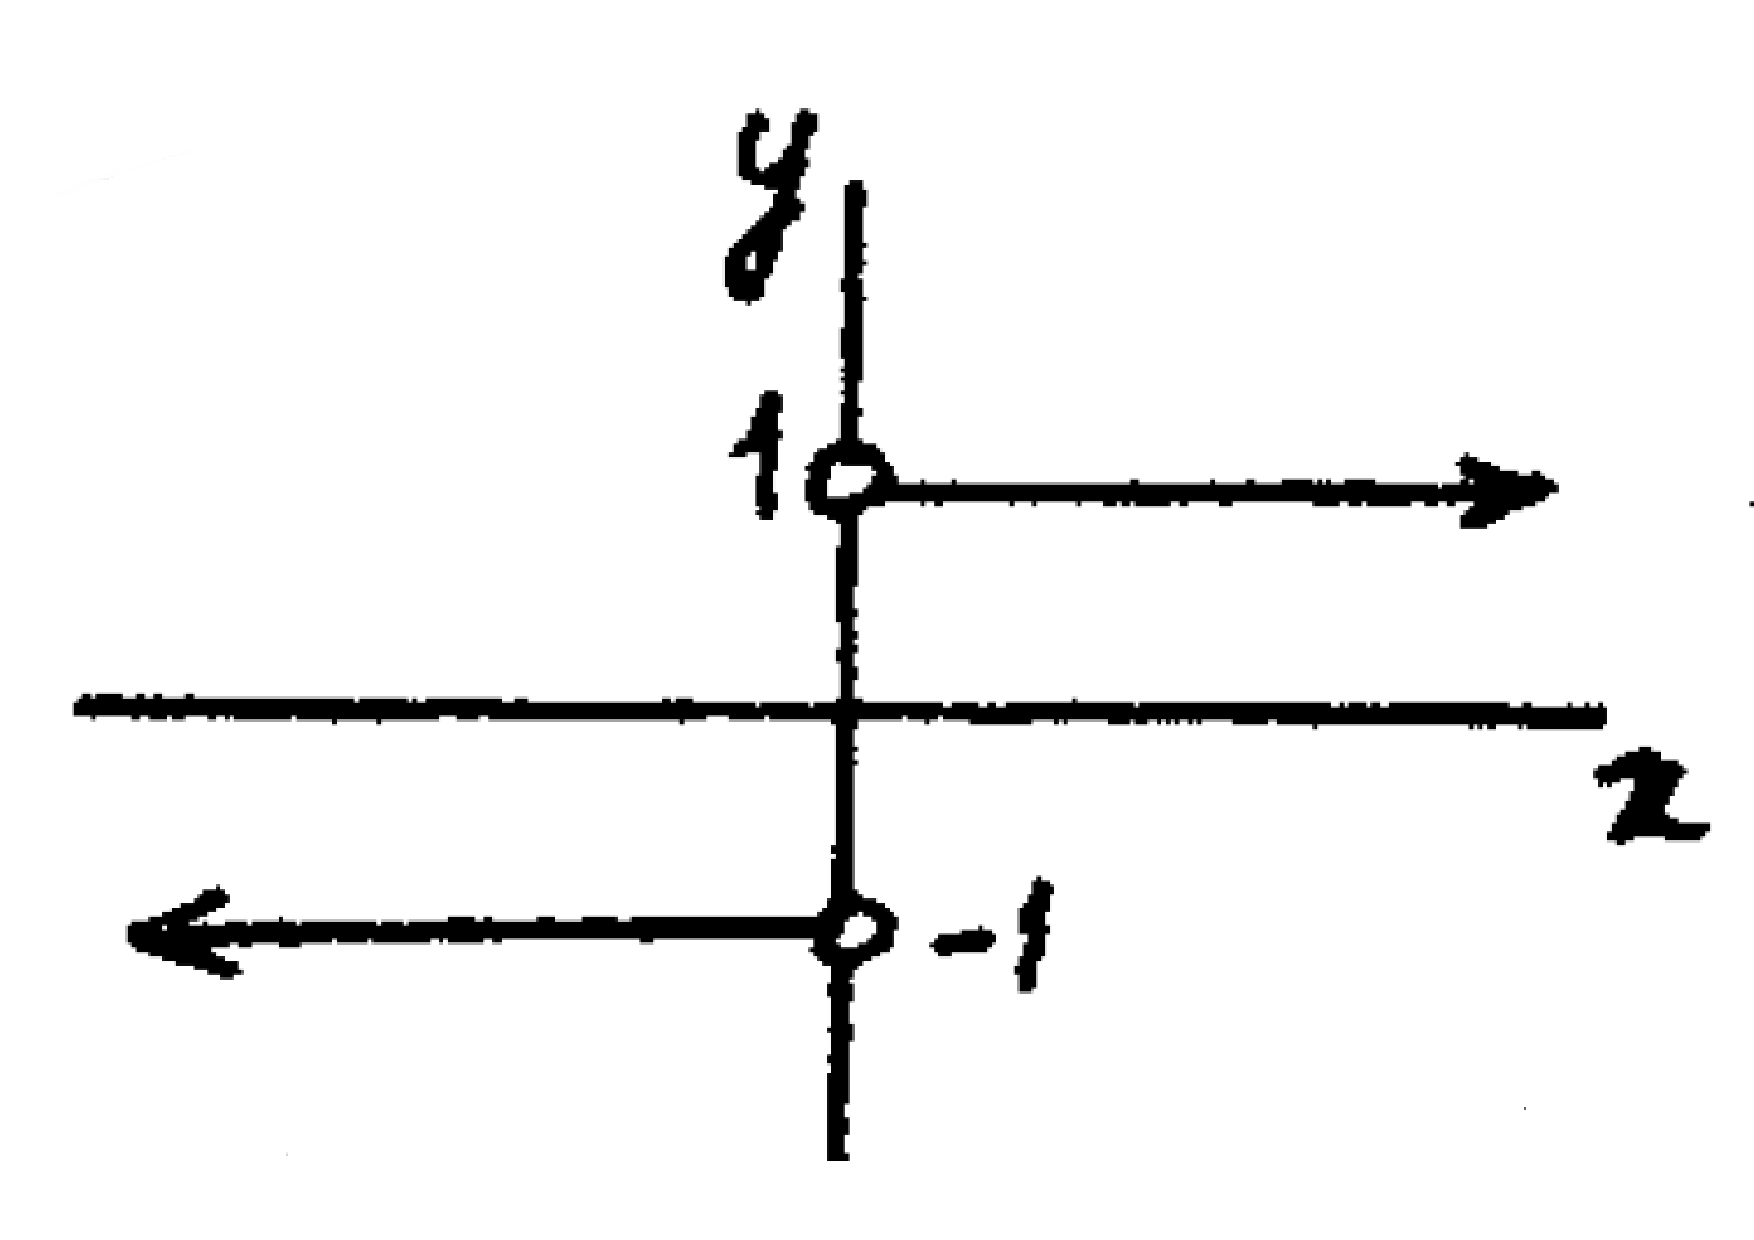
\includegraphics[width=0.45\textwidth]{images/ceyhun-001-samplePage-fig01}
	\caption{Classification of complex numbers}
	\label{fig:classificationOfComplexNumbersA}
\end{figure}

As seen in \reffig{fig:classificationOfComplexNumbersA}, this is not a good figure.


% =======================================
\subsubsection{Biraz daha şekiler}

This is the first figure.\\
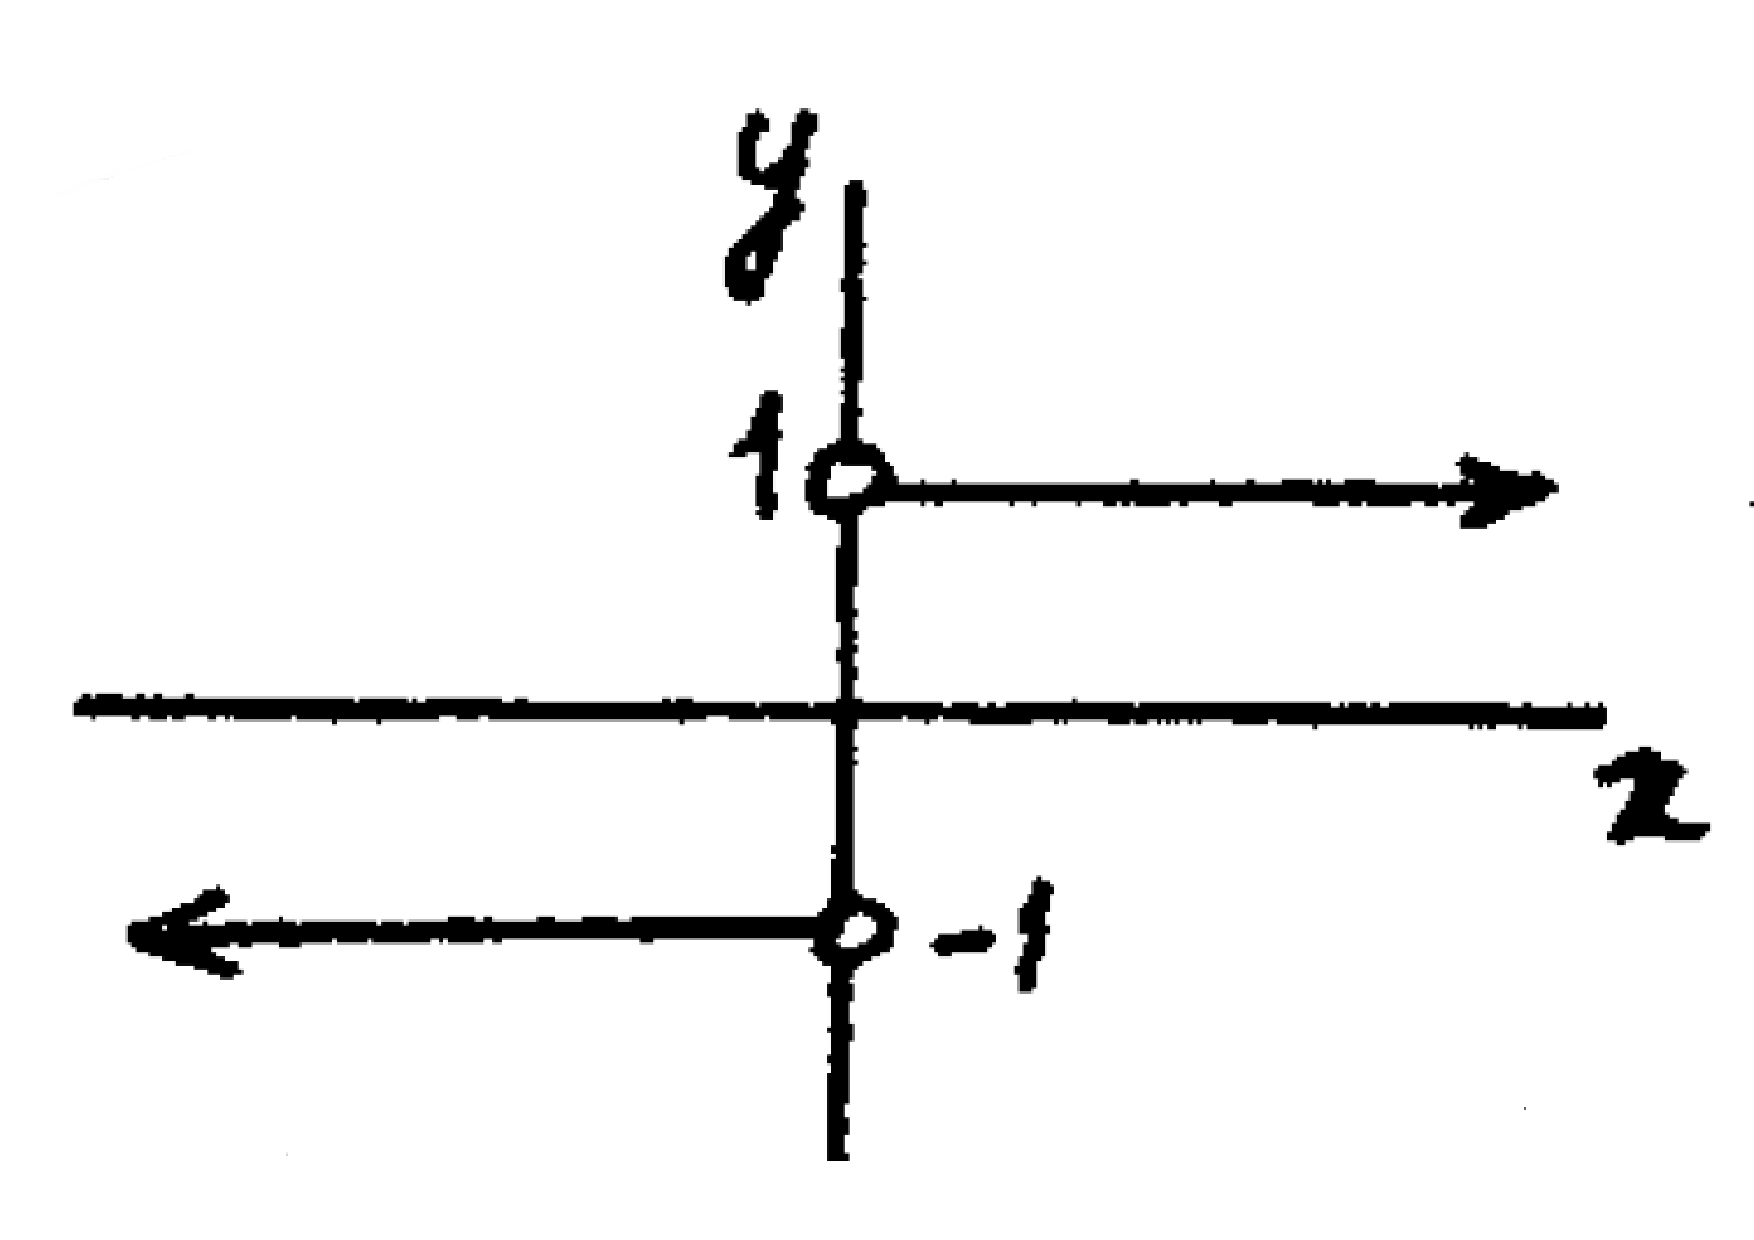
\includegraphics[width=0.45\textwidth]{images/ceyhun-001-samplePage-fig01}\\
Same more.

This is the second figure.

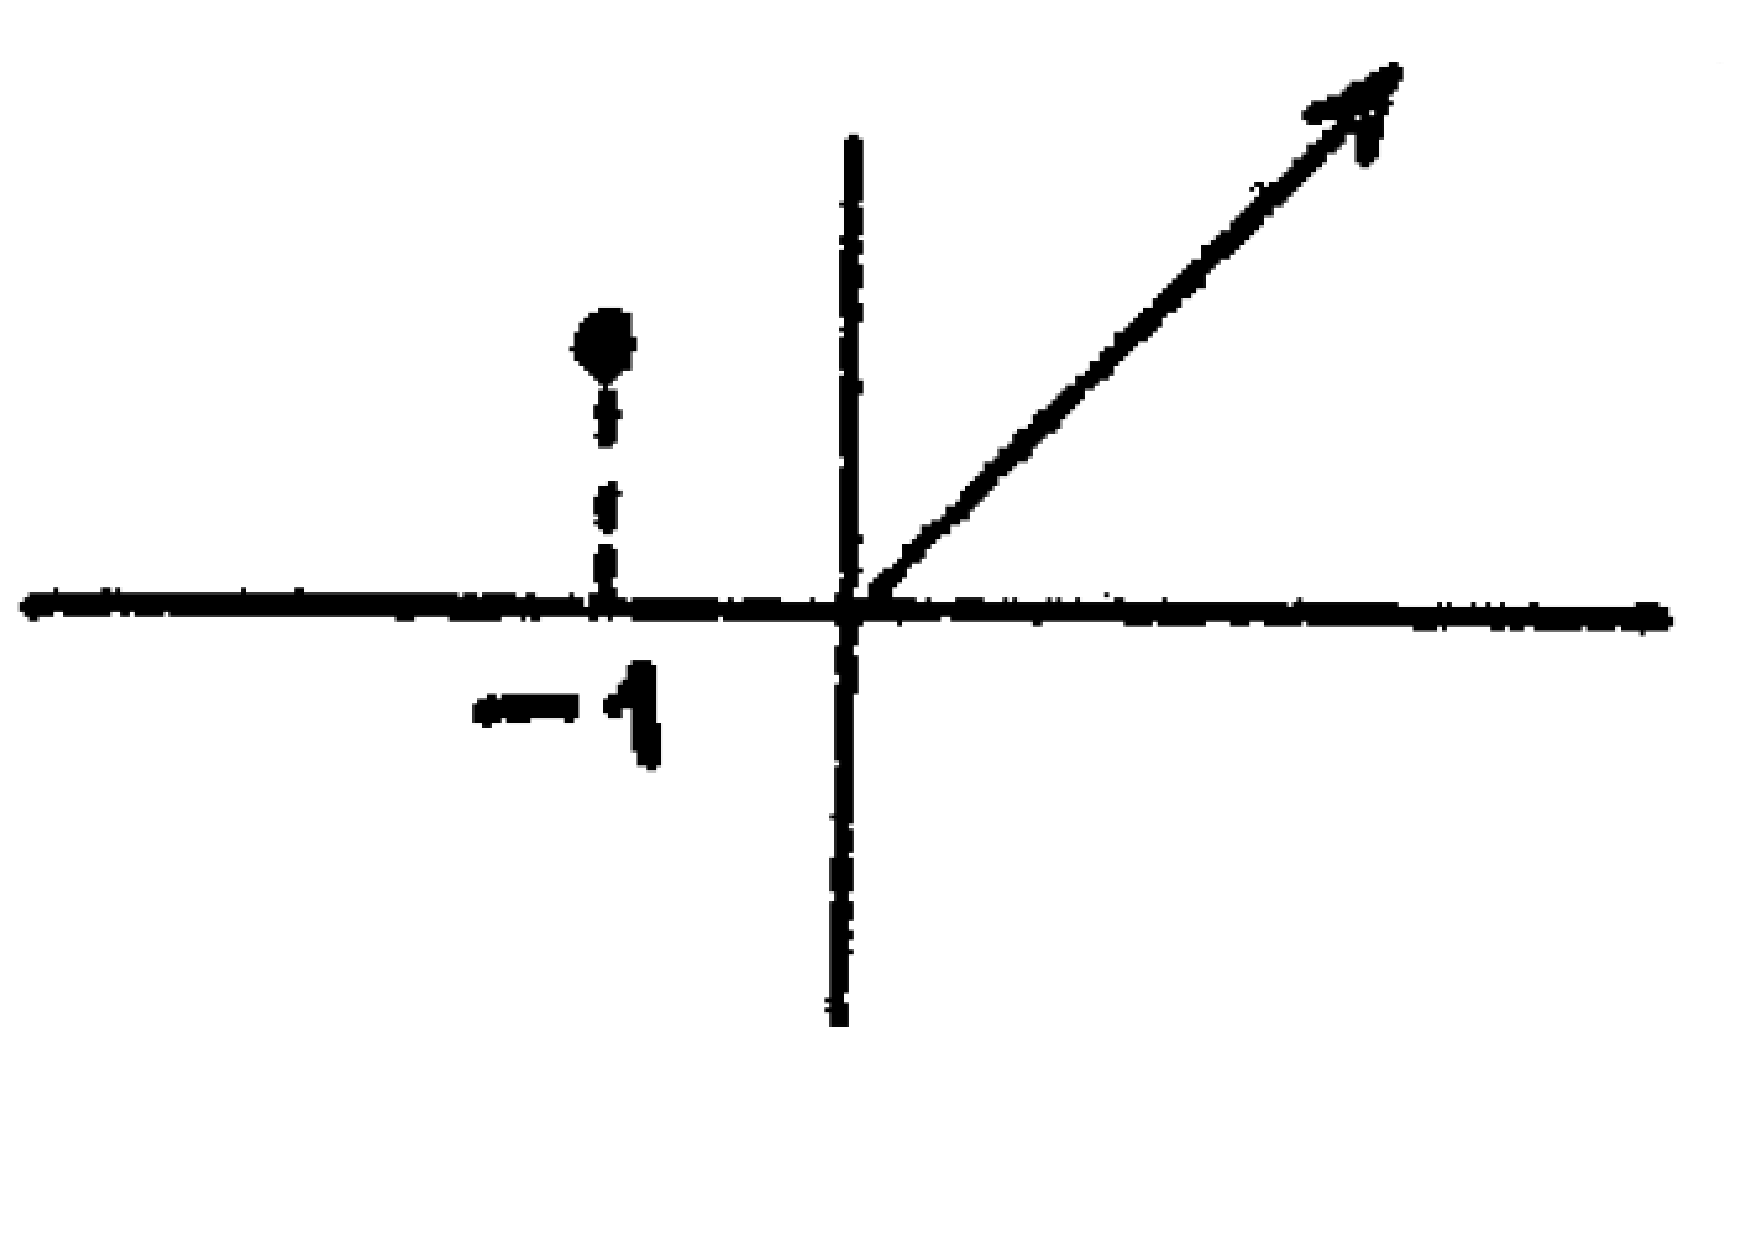
\includegraphics[width=0.45\textwidth]{images/ceyhun-001-samplePage-fig02}

Same more here, too.

Note the usage of empty line for new paragraph or usage of \verb!\\! in the \LaTeX\ code.





% =======================================================
\end{document}  

%==== templates ====

%==== environments ====

%\begin{figure}[htb]
%	\centering
%	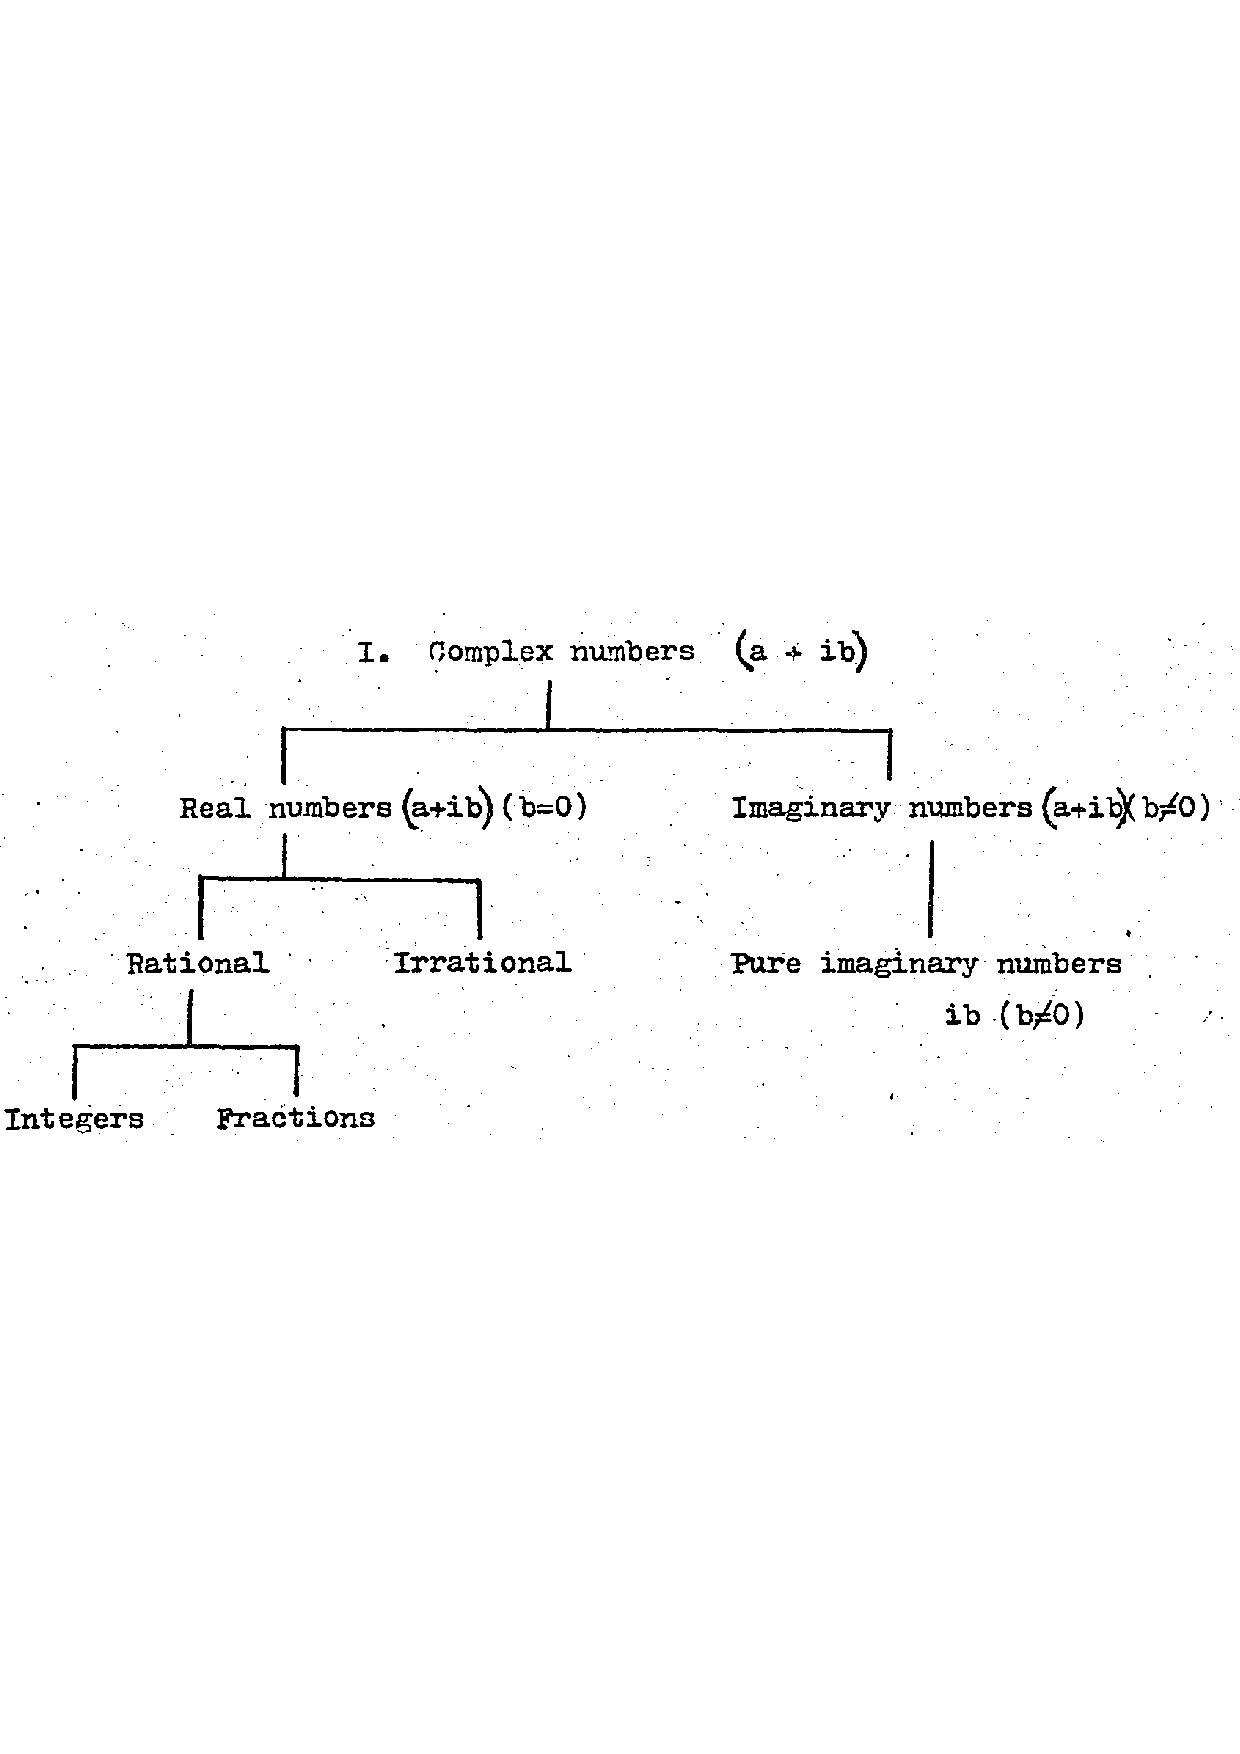
\includegraphics[width=0.9\textwidth]{images/SD-1-1p15A}
%	\caption{Classification of complex numbers}
%	\label{fig:classificationOfComplexNumbersA}
%\end{figure}

%\begin{center}
%\begin{tabular}{cc}
%\end{tabular}
%\end{center}

%\begin{exmp}
%\begin{hSolution}
%\end{hSolution}
%\end{exmp}

%\begin{hEnumerateAlpha}
%\end{hEnumerateAlpha}

%\begin{hEnumerateRoman}
%\end{hEnumerateRoman}

%$
%\begin{bmatrix}
%\end{bmatrix}
%$

%\frac{aaaa}{bbb}
%\frac{a_{n}}{b_{n}}
%\left( aaaa \right)
%\Longrightarrow

%\begin{multicols}{2}
%	bb
%\columnbreak
%	aa
%\end{multicols}
